\documentclass[norsk, 10pt, twocolumn, a4paper]{revtex4}
\usepackage[T1]{fontenc} %for å bruke æøå
\usepackage[utf8]{inputenc}
\usepackage{amsmath, amsfonts, amssymb, mathrsfs}
\usepackage{graphicx} %for å inkludere grafikk
\usepackage{verbatim} %for å inkludere filer med tegn LaTeX ikke liker
\usepackage{mathpazo}
\usepackage{listings}
\usepackage{color} %red, green, blue, yellow, cyan, magenta, black, white
\definecolor{mygreen}{RGB}{28,172,0} % color values Red, Green, Blue
\definecolor{mylilas}{RGB}{170,55,241}

\bibliographystyle{plain}

\begin{document}

\title{The Ising model and the Metropolis algorithm: \\ Ferromagnetic phase transitions \\ FYS3150 Project 4}
\author{Candidate number: 7 \\ Vilde Flugsrud}
\date{\today}

\begin{abstract}
    \center{\textbf{Abstract}}
    The aim of the project is to determine the Curie temperature $T_c$ of a system which undergoes a phase transition from ferromagnetic
    to paramagnetic when temperature is raised above a critical temperature, which corresponds to the Curie temperature. We want
    to solve the problem by modeling it with the Ising model and apply Monte Carlo methods through the Metropolis algorithm.

\end{abstract}

\maketitle

\section{Introduction}
    
    The report comprises a theory and method section followed by a result and discussion section, ending with a conclusion.
    The programes made in this project is main.cpp, isingmodel.cpp and python scripts for analysis.

\section{Theory and method}
\subsection{The physics problem}
\subsubsection{How does magnetism arise in the first place?}
Magnetism arises from two sources; electric current and the magnetic moment
induced by the spin of elementary particles, magnetic moment being a measure of the strength of a magnetic source and a
quantity which determines the torque a magnet will experience in an external magnetic field.
This project investigates the latter source. In the context of the magnetization of materials the electrons'
magnetic moments are most important, as the
magnetic moments of the nuclei is much weaker.
The electrons in a material are normally arranged such that their magnetic
moments, orbital and intrinsic, cancel out - they combine into pairs with
opposite intrinsic magnetic moments in accordance with the Pauli exclusion
principle or combine into filled subshels with no net orbital motion.
However, there are solids which may have unpaired electrons or non-filled
subshells. Whether the material produce a magnetic field is then determined
by the direction of the magnetic moments contributed by these electrons.

\subsubsection{Ferromagnetic and paramagnetic}
Ferromagnetic and paramagnetic materials are substances with such unpaired electrons.
In paramagnetic materials the magnetic moments of these tend to point in random directions,
cancelling each other out so that the material is not magnetic (in the
abcense of an external field). The magnetic moments of unpaired electrons in ferromagnetic
materials, on the other hand, have a tendency to allign parallel to one another, as this
leads to lowered energy levels. This effect makes a material magnetic, even in the absence of a
magnetic field.

\subsubsection{Phase transition}
If a ferromagnetic material is raised above a certain temperature, it loses its ferromagnetic
properties. It becomes paramagnetic as the magnetic moments of impaired electrons align
randomly, as a result of the thermal tendency to disorder (increasing entropy) becoming
stronger than the tendency towards lower energy (this drag and pull effect makes up the
thermodynamical potential Helmholtz free energy, described below).

\subsubsection{The Curie temperature}
The temperature at which a ferromagnetic substance experiences this shift is called its
Curie temperature, $T_c$. It is the critical temperature at which the system undergoes a
phase transition from ferromagnetic to paramagnetic. We now have the physics alibi for modeling
this phase transition - if done successfully it allows us to determine $T_c$.

\subsection{The canonical ensemble and the Ising model}
In order to derive the thermodynamical properties of interest, we operate with the canonical ensemble.
An ensemble is a collection of possible states a system might be in, that is it is the probability distribution for the
state of the system. The canonical ensemble describes the possible states available to a system at a fixed temperature
$T$, that is in thermal equilibrium with a heat bath. The system can exchange energy with the heat bath, meaning
the available states may differ in total energy.
This gives a probability for each microstate $i$ dependent on energy, that is $P_i = \frac{1}{Z}e^{-E_i\beta}$.
Here $\beta = \frac{1}{kT}$, $k$ being the Boltzman constant. $e^{-E_i\beta}$ is the Boltzman factor and $Z$ is the
partition function, given below.

We now introduce the Ising model which allows us to model the behaviour of the unpaired electrons'
magnetic moments in the framework of the canonical
ensemble, taking into account the interaction between neighbours.
We model the direction of the
magnetic moments of the electron spins as discrete variables which can be either $+1$ or
$-1$. The spins are arranged in a graph and allowed to interact with its neighbours.
In this project we study the two dimensional Ising model, where the graph corresponds to a
square lattic with $L$ number of spins in each direction.

Given this framework the relevant properties can be computed. We first need the partition function, the sum
of the Boltzman factor of every microstate available to the system, given as

\begin{equation}
    \label{eq:Z}
    Z = \sum\limits_{i=1}^M e^{-E_i\beta} = \sum\limits_E \Omega(E) e^{-E\beta}
\end{equation}
Where $M=2^N = 2^{L\times L}$ is the number of microstates in our two dimensional case. The first expression is a
sum over all microstates. In the second expression we see that microstates with the same
energy will have the same Boltzman factor, making it a sum over all energy levels while multiplying
the Boltzman factor with the corresponding degenerecy.

The energy of each microstate is given by

\begin{equation}
    \label{eq:Ei}
    E_i = -J\sum_{\langle kl \rangle}^N s_k s_l
\end{equation}


The energy expectation value for the canonical ensamble is given as
\begin{equation}
    \label{eq:Eexp}
    \langle E\rangle = -\frac{\delta ln Z}{\delta\beta}
    \langle E\rangle = \sum_{i=1}^M E_i P_i =\frac{1}{Z}\sum_{i=1}^M E_i e^{-E_i\beta}
\end{equation}
using the probability $P_i=\frac{1}{Z} e^{-E_i\beta}$ for a microstate $i$.

The mean magnetization of the system is

\begin{equation}
    \label{eq:Mexp}
    \langle \mathscr{M} \rangle =\sum_{i=1}^M \mathscr{M}_i P_i =\frac{1}{Z}\sum_{i=1}^M \mathscr{M}_i e^{-E_i\beta}
\end{equation}

where the magnetization of one microstate $\mathscr{M}_i$ is given as

\begin{equation}
    \label{eq:Mi}
    \mathscr{M}_i = \sum_{j=1}^N s_j
\end{equation}

that is the sum over all the $N$ spins in one configuration.

As stated earlier, the mechanisms driving the spins to parallel or random alignement is the combination of a strive
towards lower energy and higher entropy,
steered by a system's need to minimize the thermodynamical potential, which for the canonical ensemble is
the Helmholtz free energy $F$:

\begin{equation}
    \label{eq:F}
    F = \langle E \rangle - ST
\end{equation}

$S$ being the entropy.

Phase transitions may be defined as discontinuity in some order derivative of quantities related to the
thermodynamical potential of a given system.
A first order phase transition is marked by a discontinuity in the first order derivative, while a second order
phase transition is marked by a discontinuity in the second order derivative. While the expectation energy is
a first order quantity,
other thermodynamical properties such as the heat capacity $C_v$ are of the second order. This quantity is defined
\begin{align}
    \label{eq:Cv}
    C_v & = - \frac{\delta \langle E \rangle}{\delta\beta} = \frac{\delta^2 lnZ}{\delta\beta^2} \\
        & = \frac{1}{k_BT^2}\sigma_E^2
\end{align}

Where $\sigma_E^2 = \langle E^2 \rangle - \langle E \rangle^2$ is the variance, relating to
the energy fluctuations in the system.

Finally, magnetic susceptibility is given as

\begin{equation}
    \label{eq:chi}
    \chi = \frac{1}{k_BT} \sigma_{\mathscr{M}}^2= \frac{1}{k_BT}(\langle\mathscr{M}^2\rangle - \langle\mathscr{M}\rangle^2)
\end{equation}


\subsubsection{Finite size}
The Ising model has limitations of which the consequences are not neglible. In order for the theory of the canonical ensemble
to be true, we need to operate in the thermodynamical limit, that is the number of spins in each direction $L$
goes to infinity. Thus for every computation we conduct with a fixed value of $L$, we must be aware of the effects of a finite
lattice size.

The finite lattice size require us to handle the end points in the lattice. In this project we do so by periodic
boundary conditions.

\subsection{Analytical calculation $L=2$ lattice}
We first look into the properties of the Ising model analytically, for a small $L=2$ system, 
labeling the spins as $s_1$, $s_2$, $s_3$ and $s_4$ in the following
manner

\begin{align*}
%\begin{pmatrix}
  s_1 \quad s_2 \\
  s_3 \quad s_4 \\
%\end{pmatrix} 
\end{align*}

Thus the energy of a microstate for this lattice size, using equation \ref{eq:Ei}, becomes

\begin{align}
    E_i & = -J(s_1s_2 + s_2s_1 + s_1s_3 + s_3s_1 \\ 
        &+ s_2s_4 + s_4s_2 + s_3s_4 + s_4s_3)
\end{align}

Calculating the energies for the  $M= 2^N = 2^{L\times L}= 16$ microstates we find that there are three possible energies,
that is $-8J$, $0$ and $8J$. The energy $-8J$ is shared by the two microstates with all spins either up or down,
that is $\Omega(-8J)=2$. The energy $0$ is shared by the microstates of three up and one down (four states),
one up and three down (four states), and two up and two down states except the ones where equal spins are on the
diagonals (four states). Thus $\Omega(0) =12$. The energy $8J$ corresponds to the two up and two down states where
equal spins are on the diagonal (two states), giving $\Omega(8J)=2$.

Equation \ref{eq:Z} now gives the $2\times 2$ partition function

\begin{align*}
    Z & = \Omega(-8J)e^{-(-8J)\beta} + \Omega(0)e^{-0\cdot\beta} + \Omega(8J)e^{-8J\beta} \\
      & = 2e^{8J\beta} + 12 + 2e^{-8J\beta} \\
      & = \frac{1}{4}(cosh(8J\beta) + 3)
\end{align*}


From equation \ref{eq:Eexp} we find the mean energy
\begin{align*}
    \langle E\rangle = -8J \frac{sinh(8J\beta)}{3 + cosh(8J\beta)}
\end{align*}

Equations ref{eq:Mexp} and \ref{eq:Mi} gives
\begin{align*}
    \langle \mathscr{M} \rangle = 0 
\end{align*}

Calculating the expectation value of the absolute magnetization one finds
\begin{align*}
    \langle |\mathscr{M}| \rangle = 2\frac{e^{8J\beta} + 2}{cosh(8J\beta) + 3}
\end{align*}

The reason it is of interest to take the absolute value of the magnetization here is the effects of the finite lattice size.
The finite lattice size allows for jumps in the magnetization due to a change of sign which we would not see in the
thermodynamical limit.

From equation \ref{eq:Cv} we calculate the specific heat
\begin{align}
    C_v = \frac{64J^2}{kT^2}(\frac{cosh(8J\beta)}{3+cosh(8J\beta)} - \frac{sinh^2(8J\beta)}{(3+cosh(8J\beta))^2})
\end{align}

While equation \ref{eq:chi} gives the magnetic suceptibility
\begin{align*}
    \chi = \frac{8}{k_BT}\frac{e^{8J\beta}+1}{3+cosh(8J\beta)}
\end{align*}

The system's need to minimize the thermodynamical potential is what defines its equilibrium, or steady state.
Thus we start to see signs of how temperature affects the ferromangetic property of the material.
If the temperature is low, the Blotzman factor indicates that a low energy level will be highly favourable, as this
probability dominates. It leads the spins to a parallel allignement. If the temperature rises on the other hand, the
proabilities become more equal, making random allignments more probable.
It is in the steady state of the system that we are interested in observing the behaviour of the thermodynamic properties
we have defined.

\subsection{Markov chains}
In order to describe a system which moves towards a steady state or equilibrium 
given an initial configuration we introduce Markov chains.
A Markov process is a random walk with a selected probability for making
a move. In our system the random walk is the step from one spin configuration to the next.
Markov chains are in fact a discretized description of diffusion and gives a framework
for the rules of Brownian motion - the behaviour exhibited by small fractions of any system
when exposed to random fluctuations of the medium.

In order to simulate our systems evolution towards a steady state we use Markov chains
repeatidly in Monte Carlo simulations. From Markov chains we get two conditions needed
for reaching the steady state - detailed balance and ergodicity. This informs our
choice of algorithm - the Metropolis algorithm.

\subsection{Metropolis algorithm}
In order to simulate our system's evolution towards a steady state using Markov chains
we will employ the Metropolis algorithm, which meets the conditions stated above.

\begin{figure}
    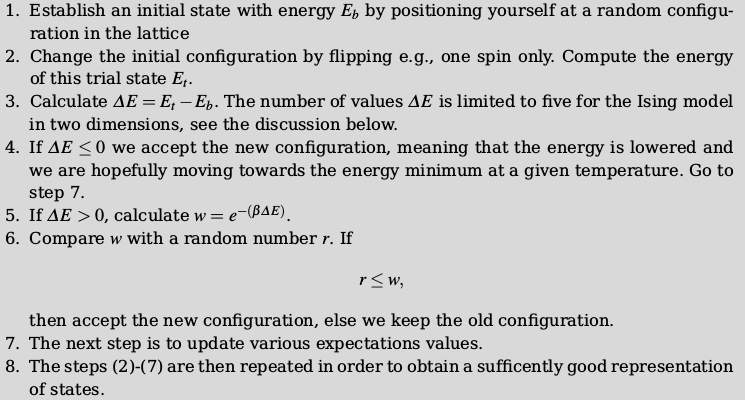
\includegraphics[width=0.9\linewidth]{metro.png}
    \caption{
        \label{fig:metro}
    The steps of the Metropolis algorithm \cite{komp}. It lets us simmulate our system's development towards
    a steady state. Computing this state for a range of temperatures we can calculate the expectation values of
    thermodynamical properties at each temperature, allowing us to observe at what temperature a phase transition might
    occur.}
\end{figure}

The steps of the Metropolis algorithm \cite{komp} are as shown in figure \ref{fig:metro}.
We decide the number of repetitions of step two to seven "in order to achieve a sufficiently good representation"
by the size of the lattice. By repeating the steps $N=L\times L$ times we allow for a maximum of N possible flips.
Thus our model scales according to the lattice size. In our model we view one Monte Carlo cycle as one time step,
and so it is natural that more spin flips occur in one time step for a bigger system.

Observe that we flip one spin at the time, if accepted we compute the corresponding change of expectation values.
After one complete sweep of the lattice, we measure the new expectation values due to these changes.
As stated, there are a limited set of energy changes available, this follows from the outline of the Ising model
in two dimensions in the previous section. The possible changes are $\Delta E=8J, 4J, 0, -4J, -8J$.

The algorithm determines whether a proposed move is implemented based on a transition probability and an
acceptance probability. The strength of the algorithm is that the transition probability need not be known.
In our case we are relieved from computing the partition function $Z$ for each proposed spin flip.
In fact the acceptance of a flip need only depend on the change in energy - if the energy becomes smaller we
accept with a probability of one, else we compute the Boltzman factor for the energy difference and compare it
to a random number.

\subsection{Code}
The code I have written implements the Metropolis algorithm
as stated above and writes the thermodynamical quantities of interest to an output file specified by the user.
This is read by a python script which plots the quantities of interest.

I made two versions of the code. The first is primarily for testing the quality of model and code.
The test this code allows for include: does the
$L=2$ case reproduce the analytical results found earlier? At what point is it safe to say that
the system has reached equlibrium so that we can measure expectation values
(we call this thermalization)?
How is it in our interest to look at the absolute value of the magnetization? Should it extend to our definition
of the magnetic suceptibility?
Does the number of spin flips it accepts seem reasonable? 
With which probabilities does it actually produce different energy levels at different temperatures?
Results of such tests can be seen in the following section.

The second version of the code implements these findings to the end of giving the best possible representation of our system.
Some decisions made in this code is to start with an ordered configuration at low temperatures and random at higher temperatures
assuming these are the more likely states leading quicker to thermalization. Thermalization is accepted at the point where
$\langle E\rangle$ and $C_v$ has changed less than $5\%$ since the previous measurement.
the time needed to reach a steady state is longer for temperatures close
to the critical temperature than for temperatures away.

Furthermore, the second version parallelizes the computation of temperatures using MPI. Thus, this is the code used to finally
model how the thermodynamical properties develop as we increase temperature. I ran the code for a number of 1 million Monte Carlo
cycles using two processors on a laptop with one CPU. 
Please see the codes for further comments and details.


\subsection{Phase transition and how to find $T_c$}
In order to compute the actual $T_C$ corresponding to the thermodynamical limit from our $T_c$ restricted by the lattice size, we
make use of the followin relation

\begin{align}
    T_c(L=\infty) = T_c(L) - aL^{-\frac{1}{\nu}}
\end{align}
where the exact result gives $\nu=1$ and $a$ is a constant. 

\section{Results and discussion}
\subsection{Computations compared with analytical}
\begin{figure}
    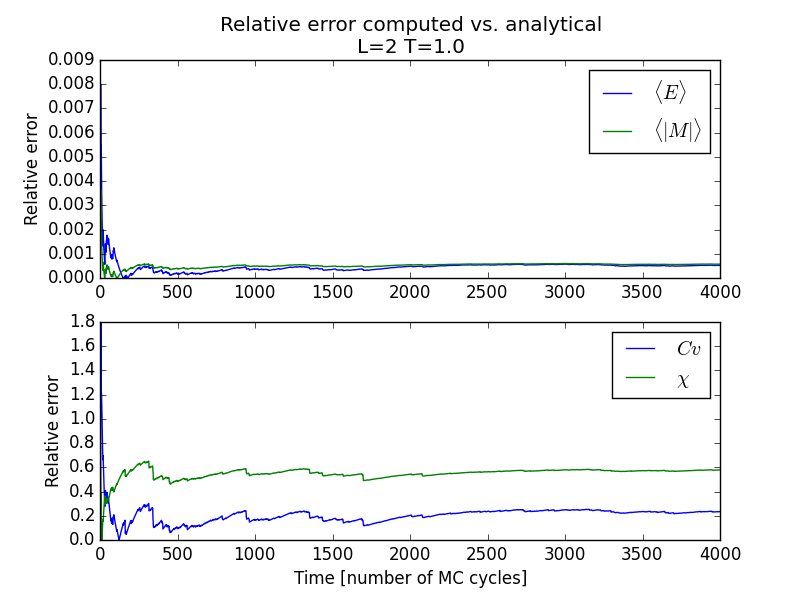
\includegraphics[width=0.9\linewidth]{error.png}
    \caption{
        \label{fig:b1}
        The relative error of the computed thermodynamical quantities vs the analytical values.
    The error is small, indicating that the code is functional.}
\end{figure}
The relative error is plotted in figure \ref{fig:b1}. There is a good agreement and
stabilization of the error at a $10^3$ number of Monte Carlo cycles.

\subsection{Thermalization and rate of acceptance}
\begin{figure}
    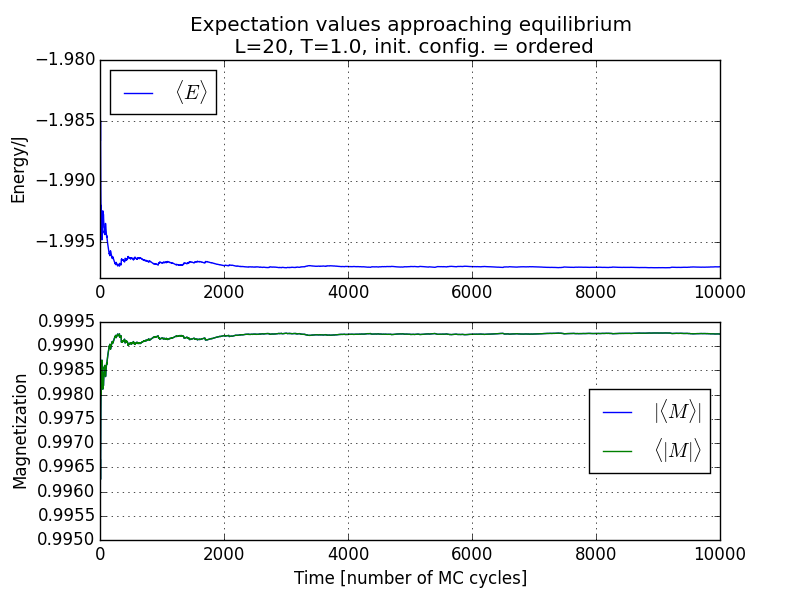
\includegraphics[width=0.9\linewidth]{c_ordered_L20t1mcE4.png}
    \caption{
        \label{fig:c1}
        The graph shows how the magnetization and the energy of the system evolves with time,
    that is the number of Monte Carlo cycles in the simulation}
\end{figure}
\begin{figure}
    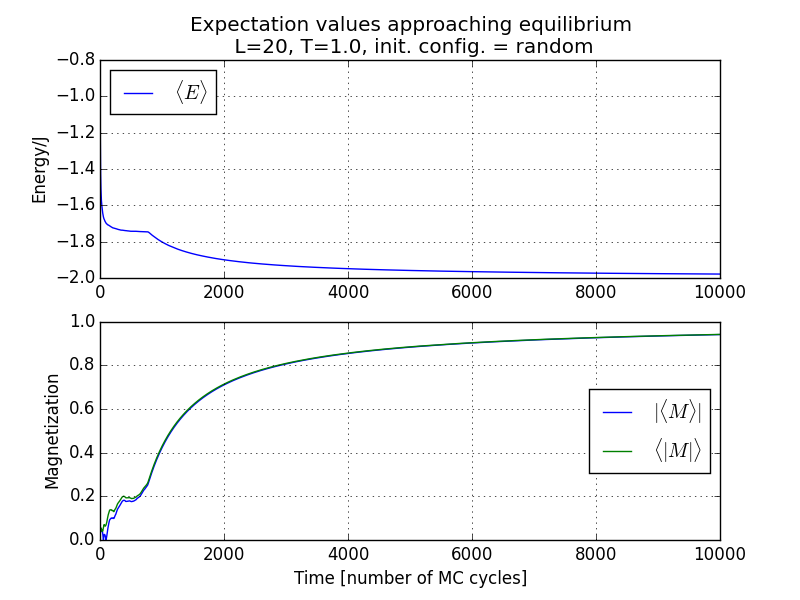
\includegraphics[width=0.9\linewidth]{c_random_L20t1mcE4.png}
    \caption{
        \label{fig:c2}
        The graph shows how the magnetization and the energy of the system evolves with time,
        that is the number of Monte Carlo cycles in the simulation.}
\end{figure}
\begin{figure}
    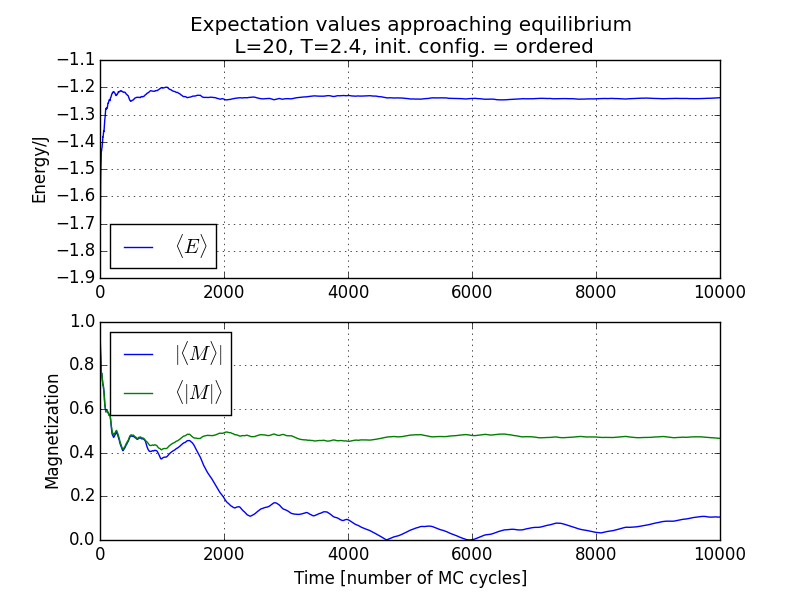
\includegraphics[width=0.9\linewidth]{c_ordered_L20t24mcE4.png}
    \caption{
        \label{fig:c3}
        The graph shows how the magnetization and the energy of the system evolves with time,
        that is the number of Monte Carlo cycles in the simulation.}
\end{figure}
\begin{figure}
    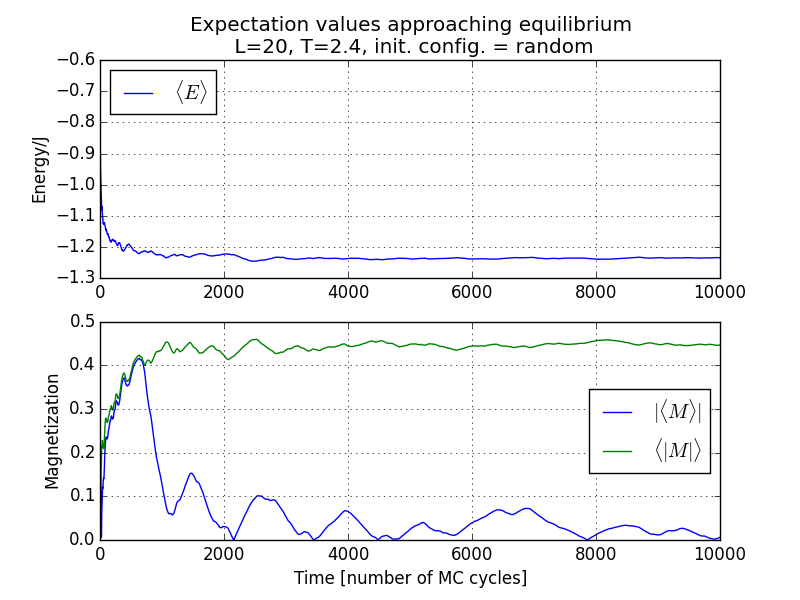
\includegraphics[width=0.9\linewidth]{c_random_L20t24mcE4.png}
    \caption{
        \label{fig:c4}
        The graph shows how the magnetization and the energy of the system evolves with time,
        that is the number of Monte Carlo cycles in the simulation.}
\end{figure}

\begin{figure}
    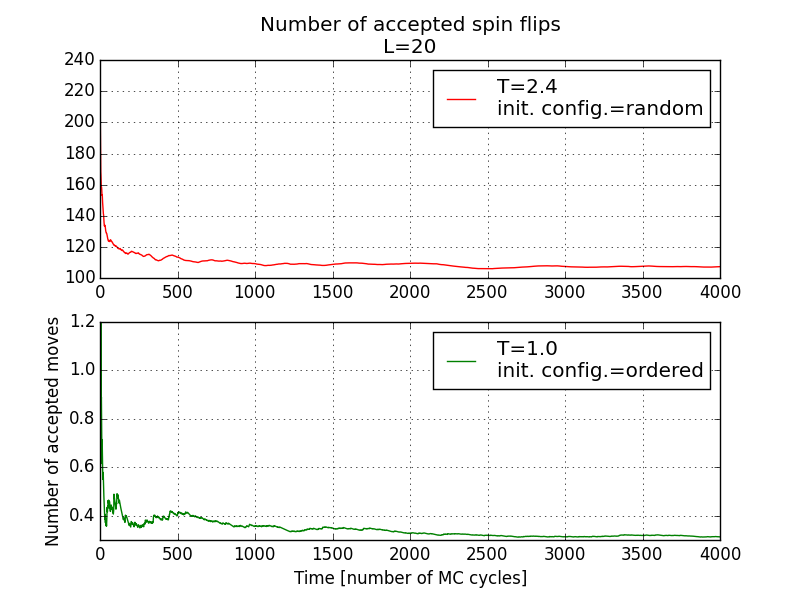
\includegraphics[width=0.9\linewidth]{c_accepted.png}
    \caption{
        \label{fig:c5}
        This graph shows the number of spins in our model flipped over time at two different
    temperatures.}
\end{figure}

See figures \ref{fig:c1}, \ref{fig:c2}, \ref{fig:c3} and \ref{fig:c4} for the expectation values plotted against time.
We first notice that the expectation values take on the expected values, for example the energy
is lowest energy level, $-2$ per spin, at the low temperature. Furthermore, we see how the
different two different computations of the absolute magnetization differs.
We see that  $\\langle |\mathscr{M}| \\rangle$ has the smoothest graph, this is our motivation
for calculating the suceptibility later on with this value. It is "cheating" in order
to avoid some unwanted effects of our finite lattice.

Finally we see why we want to put in the test of thermalization - the system clearly needs
to reach the steady state before we start measurements, or else our expectation values will
be skewed.

See figure \ref{fig:c5} for the plot of accepted moves against time. While few moves are
accepted at a low temperature, many more, (about $30\%$) are accepted at $T=2.4$.
This is as we would expect above and below the critical temperature.

\subsection{P(E)}
\begin{figure}
    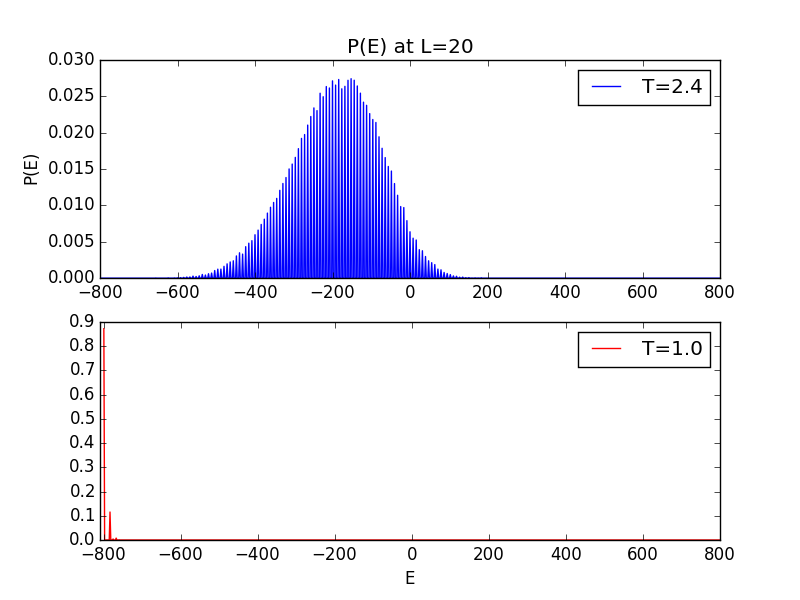
\includegraphics[width=0.9\linewidth]{E_count.png}
    \caption{
        \label{fig:d1}
        Exp}
\end{figure}
See figure \ref{fig:d1}. For the energy probabilites. Again it corresponds to what we know
about the ferromagnetic material. The variance of E was computed as 9 for low $T$ and
3283 for high $T$. As the standard deviation is the squareroot of this, meaning energy values
are mostly the same at the low temperature and spread out over a wider range of levels at the
higher temperature, these are good results.

\subsection{Phase transition}
\begin{figure}
    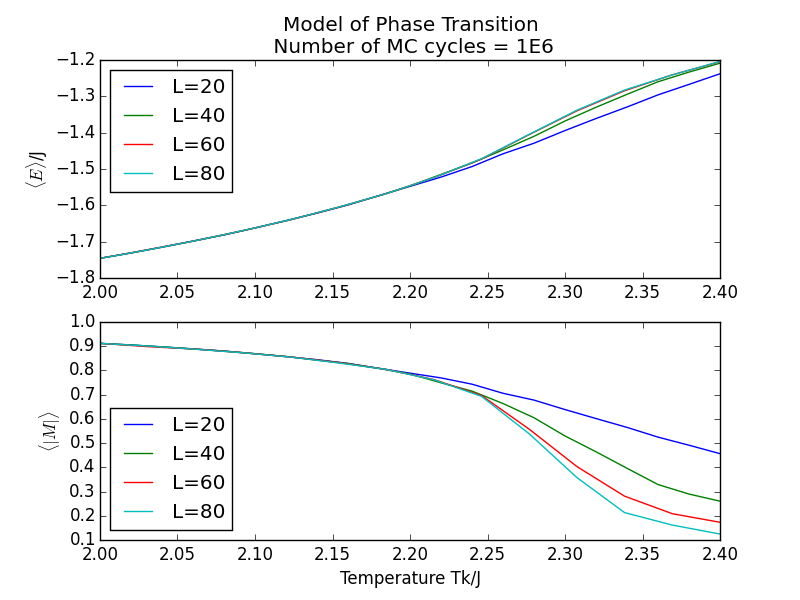
\includegraphics[width=0.9\linewidth]{e1.png}
    \caption{
        \label{fig:e1}
        Behaviour of energy and magnetism during the phase transition}
\end{figure}
\begin{figure}
    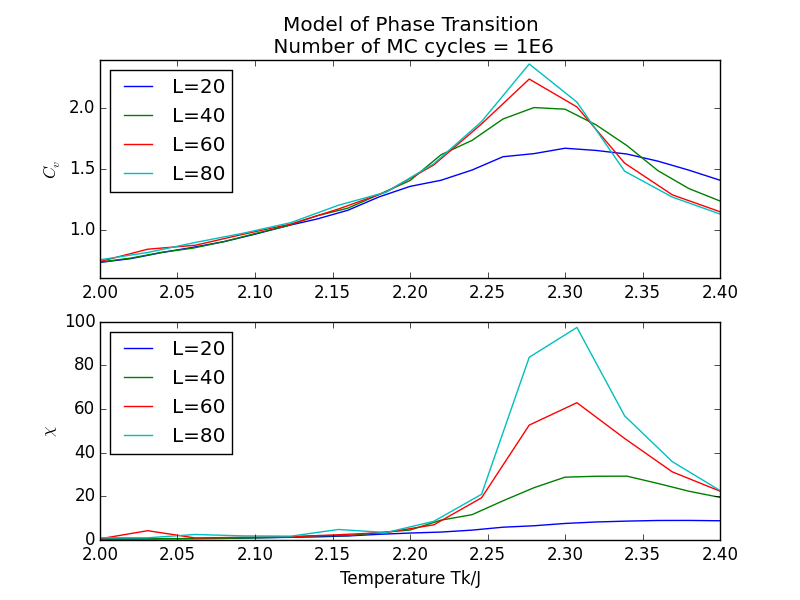
\includegraphics[width=0.9\linewidth]{e2.png}
    \caption{
        \label{fig:e2}
        Behaviour of specific heat and magnetic suceptibility during phase transition}
\end{figure}
See figures \ref{fig:e1} and \ref{fig:e2}.
We clearly see the signs of the transition - the slope of the energy is steeper,
the magnetism is about to disappear (but never really does due to our finite lattice size),
and the specific heat and suceptibility peak. This all happen around $2.3$, which is close
to the expected value $2.69$. As we saw in the equation relating the finite lattice result to
the actual $T_c$, the two become closer as $L$ increases, and we see this effect in these figures.

\section{Conclusion}
In this project we used the Ising model and the Metropolis algorithm to model the phase transition
from ferromagnetic to paramagnetic material. In this we tried to obtain the Curie temperature.
This was successful as the model exhibited a phase transition around $2.3$, the exact result
being $2.69$. For future work one could look into models that differ from the Ising and Metropolis methods
- for example methods of flipping several spins at a time, seeing a quicker development of the heat
capacity near the critical temperature.


\section{Appendix}


\begin{thebibliography}{1}
\bibitem{komp} M. Hjort-Jensen {\em Computational Physics: Lecture Notes}  UiO 2015.

\end{thebibliography}

\end{document}

